\documentclass[11pt]{article}

\usepackage[margin=0.85in]{geometry}
\usepackage{amsmath}
\usepackage{booktabs}
\usepackage{enumitem}
\usepackage{float}
\usepackage{graphicx}
\usepackage{hyperref}
\usepackage{microtype}
\usepackage{multirow}
\usepackage{pgfplots}
\usepackage{tikz}
\usepackage{xcolor}
\usetikzlibrary{arrows.meta, positioning, shapes.geometric, fit, backgrounds}
\pgfplotsset{compat=1.18}

\definecolor{inputblue}{HTML}{DCEEFF}
\definecolor{planpurple}{HTML}{E9DDFC}
\definecolor{execgreen}{HTML}{DFF2E1}
\definecolor{checkorange}{HTML}{FCE6CC}
\definecolor{healred}{HTML}{F8D7DA}
\definecolor{darkblue}{HTML}{174A7E}

\hypersetup{
    colorlinks=true,
    linkcolor=darkblue,
    citecolor=darkblue,
    urlcolor=darkblue
}

\title{\textbf{Agent-Oriented Query Planning over a Financial Knowledge Graph:}\\
A Comparative Study of Hybrid and Local Language-Model Pipelines}
\author{Anonymous Author(s)\\
\small Draft prepared from the \texttt{financial/aop\_general\_300\_mismatch} experiments}
\date{\today}

\begin{document}
\maketitle

\begin{abstract}
This paper presents an engineering study of an agent-oriented pipeline (AOP) for answering natural-language financial questions over an RDF knowledge graph. Relational financial data were represented as RDF instances aligned with an ontology, and language models were assigned modular roles for schema retrieval, query classification, directed acyclic graph (DAG) planning, SPARQL generation, validation, self-healing, and answer explanation. We evaluate three completed configurations on the same 300 previously mismatched questions: (i) a hybrid GPT-5.2 planner and SPARQL generator with Qwen2.5-Coder-14B semantic operators, (ii) an all-local Qwen2.5-Coder-14B pipeline with Qwen2.5-Coder-32B grading, and (iii) a hybrid GPT-5.2 planner and SPARQL generator with Gemma-4-26B semantic operators. The Gemma hybrid produced 100 exact matches, 130 partial matches, and 70 mismatches, compared with 86/119/95 for the Qwen hybrid and 85/103/112 for all-local Qwen. The results indicate that stronger semantic operators reduce scan errors and self-healing demand, while stronger planning and SPARQL generation primarily improve robustness rather than exact-match accuracy. We also document alias normalization, deterministic graph validation, resumable evaluation, and failure modes that materially affected the study. Because model routing, final graders, and alias-map revisions were not fully controlled across all runs, the findings should be interpreted as an engineering evaluation rather than a definitive model leaderboard.
\end{abstract}

\section{Introduction}

Financial analytics systems commonly use relational databases because aggregation, filtering, and joining are naturally expressed in SQL. However, relational schemas can become difficult to reuse when data originate from multiple systems, use inconsistent identifiers, or require reasoning across semantically related entities. Knowledge graphs (KGs) address this problem by representing entities, attributes, and relations in a shared graph model \cite{hogan2021kg}. RDF provides a standardized representation, while SPARQL provides a query language over RDF graphs \cite{rdf11,sparql11}.

This work investigates whether an agent-oriented pipeline can translate natural-language questions into reliable KG queries. The system does not perform a single monolithic model call. Instead, it decomposes the task into operators such as \textit{Retrieve}, \textit{Classify}, \textit{Generate}, \textit{Scan}, \textit{Validate}, and \textit{Explain}. A language-model planner proposes an execution DAG; deterministic Python code validates and executes the graph; and a self-healing loop regenerates SPARQL when query execution fails or returns an invalid result.

The study asks four practical questions:

\begin{enumerate}[leftmargin=*]
    \item Can a modular AOP reliably answer previously failed financial KG questions?
    \item How do hybrid GPT/local-model configurations compare with an all-local Qwen configuration?
    \item Which optimizations reduce failures caused by malformed DAGs, hallucinated RDF terms, and identifier mismatches?
    \item Where do remaining errors originate: planning, schema grounding, SPARQL generation, graph execution, explanation, or grading?
\end{enumerate}

\section{Background and Related Work}

\subsection{Knowledge Graphs, RDF, and SPARQL}

Knowledge graphs encode entities and their relationships using a graph-oriented representation. RDF represents statements as subject--predicate--object triples \cite{rdf11}. SPARQL supports graph-pattern matching, filtering, aggregation, optional patterns, negation, and ordering over RDF datasets \cite{sparql11}. Compared with a fixed relational schema, an ontology-backed KG provides explicit semantic types and relationships that can support cross-source integration and multi-hop reasoning. This flexibility comes at a cost: generated SPARQL must use the exact classes, properties, identifiers, and relationship directions present in the graph.

\subsection{Agent-Oriented Pipelines}

Agent-oriented programming treats agents, capabilities, messages, and commitments as primary abstractions \cite{shoham1993aop}. Modern language-model agents operationalize related ideas by interleaving reasoning with actions or tool calls. ReAct demonstrated that language models can combine reasoning traces with external actions to improve knowledge-intensive and interactive tasks \cite{yao2023react}. Our system follows this modular spirit: semantic operators are model-powered, while graph querying and structural checks are deterministic tools.

\subsection{Iterative Repair and Self-Healing}

Iterative self-feedback has been studied as a way to improve language-model outputs without additional training \cite{madaan2023selfrefine}. Our self-healing loop differs from unconstrained textual refinement: failed SPARQL is paired with execution diagnostics, unknown RDF terms, candidate replacements, and properties observed in the graph. The model is then asked to regenerate an executable query using the newly exposed evidence.

\subsection{Text-to-Query Evaluation}

Text-to-SQL benchmarks such as Spider emphasize generalization across databases and schemas \cite{yu2018spider}. Our setting is related but targets SPARQL over an ontology-aligned RDF graph. Importantly, this paper does not claim that KG querying is superior to SQL for simple aggregation. Rather, it studies the engineering trade-offs of a semantic execution layer, dynamic planning, and recovery across heterogeneous model configurations.

\section{System Architecture}

\subsection{End-to-End Pipeline}

Figure~\ref{fig:pipeline} summarizes the implemented pipeline.

\begin{figure}[H]
\centering
\resizebox{\textwidth}{!}{
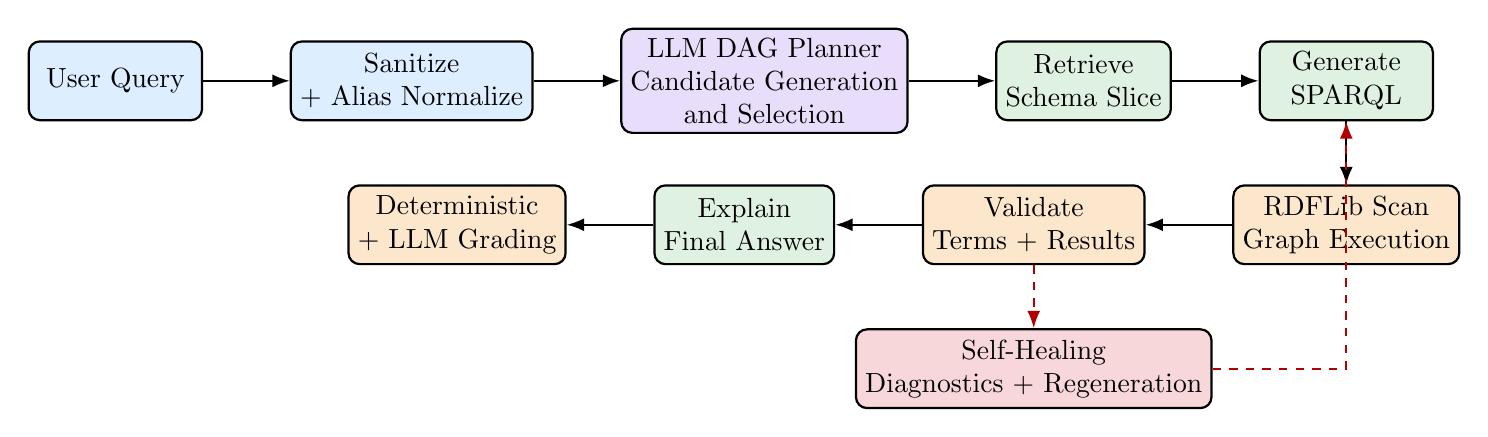
\begin{tikzpicture}[
    node distance=8mm and 11mm,
    box/.style={rectangle, rounded corners, draw, thick, align=center, minimum height=10mm, minimum width=22mm},
    arrow/.style={-{Latex[length=2.2mm]}, thick},
    retry/.style={-{Latex[length=2.2mm]}, thick, dashed, red!70!black}
]
\node[box, fill=inputblue] (query) {User Query};
\node[box, fill=inputblue, right=of query] (prep) {Sanitize\\+ Alias Normalize};
\node[box, fill=planpurple, right=of prep] (planner) {LLM DAG Planner\\Candidate Generation\\and Selection};
\node[box, fill=execgreen, right=of planner] (retrieve) {Retrieve\\Schema Slice};
\node[box, fill=execgreen, right=of retrieve] (generate) {Generate\\SPARQL};
\node[box, fill=checkorange, below=of generate] (scan) {RDFLib Scan\\Graph Execution};
\node[box, fill=checkorange, left=of scan] (validate) {Validate\\Terms + Results};
\node[box, fill=execgreen, left=of validate] (explain) {Explain\\Final Answer};
\node[box, fill=checkorange, left=of explain] (grade) {Deterministic\\+ LLM Grading};
\node[box, fill=healred, below=of validate] (heal) {Self-Healing\\Diagnostics + Regeneration};

\draw[arrow] (query) -- (prep);
\draw[arrow] (prep) -- (planner);
\draw[arrow] (planner) -- (retrieve);
\draw[arrow] (retrieve) -- (generate);
\draw[arrow] (generate) -- (scan);
\draw[arrow] (scan) -- (validate);
\draw[arrow] (validate) -- (explain);
\draw[arrow] (explain) -- (grade);
\draw[retry] (validate) -- (heal);
\draw[retry] (heal.east) -| (generate.south);
\end{tikzpicture}}
\caption{Implemented agent-oriented KG question-answering pipeline. Dashed arrows denote the self-healing retry loop.}
\label{fig:pipeline}
\end{figure}

\subsection{Operator Registry}

The planner chooses from semantic and deterministic operators:

\begin{itemize}[leftmargin=*]
    \item \textbf{Semantic operators:} Retrieve, Classify, Link, Extract, Generate, Refine, Validate, Filter\_Aggregate, Order\_By, Integrate, and Explain.
    \item \textbf{Deterministic operators:} Check\_Schema, Scan, Math\_Compute, Set\_Intersect, Set\_Union, and Set\_Difference.
\end{itemize}

The core execution path is generally
\[
\text{Retrieve} \rightarrow \text{Generate} \rightarrow \text{Scan}
\rightarrow \text{Validate} \rightarrow \text{Explain}.
\]
For aggregation or numeric-superlative questions, \textit{Classify} is normally inserted before \textit{Generate}. Optional operators may form additional branches when the planner judges them useful.

\subsection{DAG Planning and Validation}

The planner generates multiple linear candidate plans, rewrites unique candidates as node/edge JSON, and builds a NetworkX DAG. Python performs authoritative structural validation:

\begin{enumerate}[leftmargin=*]
    \item the graph must be acyclic;
    \item mandatory operators must be present;
    \item required dependency paths must connect Retrieve, Generate, Scan, Validate, and Explain;
    \item Classify must precede Generate when required; and
    \item Explain must terminate execution.
\end{enumerate}

The language-model reward evaluator scores only semantic efficiency and optional-operator usefulness. A Python-valid DAG receives a score floor of 0.5, preventing an LLM judge from falsely rejecting a structurally correct graph. No manual fallback DAG is used in the principal experiments.

\subsection{Knowledge Graph Construction}

The instance graph is stored in \texttt{business\_data\_kg\_schema\_aligned.ttl}; ontology/schema metadata are loaded from \texttt{schema\_linkage\_graph\_v2.rdf}. Runtime schema extraction produced 119 classes with dynamically observed properties and datatypes. RDFLib executes generated SPARQL locally.

\section{Engineering Optimizations}

\subsection{Schema Retrieval and Prompt Reduction}

The Retrieve operator receives a lightweight class/property index and selects a schema slice relevant to the question. Generate receives the slice rather than the full schema when retrieval succeeds. If no valid class is returned, the full dynamic schema is used as a fallback context. This optimization reduces prompt size but introduces a retrieval-recall trade-off.

\subsection{RDF-Derived Alias Resolution}

Identifier mismatch was a recurring failure source. A shared alias map is generated directly from RDF subjects, RDF objects, and ID-valued literals. The map contains 200 canonical keys after optimization. For a graph ID such as \texttt{INV001}, safe variants include:

\[
\{\texttt{INV1},\texttt{INV-1},\texttt{INV01},\texttt{INV-01},
\texttt{INV001},\texttt{INV-001}\}.
\]

Aliases are applied twice:

\begin{enumerate}[leftmargin=*]
    \item \textbf{Preprocessing:} normalize user identifiers before retrieval, planning, and SPARQL generation.
    \item \textbf{Post-generation:} normalize compact identifiers inside generated SPARQL before graph execution.
\end{enumerate}

Ambiguous aliases are retained as ambiguous and are not automatically replaced.

\subsection{Generic SPARQL Normalization}

Earlier experiments contained a large set of query-specific replacement rules. These were removed to avoid encoding answers or dataset-specific repairs in the pipeline. The current generic normalization:

\begin{itemize}[leftmargin=*]
    \item removes Markdown code fences;
    \item adds missing namespace prefixes;
    \item normalizes compact KG IDs through the RDF-derived alias map; and
    \item validates \texttt{ex:} terms against terms observed in the graph.
\end{itemize}

\subsection{Self-Healing}

When Scan fails, returns zero rows in a suspicious context, or Validate detects a problem, the pipeline collects:

\begin{itemize}[leftmargin=*]
    \item the failed SPARQL query;
    \item parser or execution errors;
    \item unknown RDF terms and close matches;
    \item actual properties observed on matched graph nodes; and
    \item a structured hint for regeneration.
\end{itemize}

Generate then rewrites the SPARQL using this feedback and Scan is executed again.

\subsection{Evaluation Reliability}

The evaluation harness provides:

\begin{itemize}[leftmargin=*]
    \item stable \texttt{Sample Row ID} values for duplicate questions;
    \item atomic CSV writes using a temporary file and \texttt{os.replace};
    \item resume behavior that preserves completed rows and retries crashes;
    \item per-query elapsed time and execution traces;
    \item deterministic fact comparison before invoking an LLM grader; and
    \item explicit trace columns for DAG sequence, SPARQL, raw rows, validation, and self-healing.
\end{itemize}

\section{Experimental Design}

\subsection{Question Set}

The evaluation set contains 300 rows sampled from questions previously marked \texttt{MISMATCH} in the broader analysis workbook. The CSV contains 232 unique question strings and 68 duplicate occurrences. Duplicate rows are intentionally retained because the evaluation unit is the sampled row, not only the unique text.

\subsection{Configurations}

\begin{table}[H]
\centering
\small
\caption{Evaluated model-routing configurations.}
\label{tab:configs}
\begin{tabular}{p{2.9cm}p{2.5cm}p{2.6cm}p{2.8cm}p{2.5cm}}
\toprule
\textbf{Configuration} & \textbf{DAG Planner} & \textbf{SPARQL Generate} & \textbf{Semantic Operators} & \textbf{Final LLM Grader}\\
\midrule
Qwen14 Hybrid & GPT-5.2 & GPT-5.2 & Qwen2.5-Coder-14B & Qwen2.5-Coder-32B\\
Qwen14 All-Local & Qwen2.5-Coder-14B & Qwen2.5-Coder-14B & Qwen2.5-Coder-14B & Qwen2.5-Coder-32B\\
Gemma26 Hybrid & GPT-5.2 & GPT-5.2 & Gemma-4-26B & Gemma-4-26B\\
\bottomrule
\end{tabular}
\end{table}

All configurations use the same RDF graph, schema extraction, deterministic operators, 300-row sample, and status taxonomy. The principal statuses are:

\begin{itemize}[leftmargin=*]
    \item \textbf{MATCH:} all required ground-truth facts are present;
    \item \textbf{PARTIAL:} some required facts are present, or strict comparison detects missing details;
    \item \textbf{MISMATCH:} the answer is unsupported, contradictory, empty, or materially different; and
    \item \textbf{CRASH:} the pipeline raises an unrecovered exception.
\end{itemize}

\subsection{Metrics}

We report exact matches, partial matches, mismatches, mean and median latency, scan-error count, number of rows requiring self-healing, mean self-healing attempts per row, and no-data/error outputs. We additionally perform paired comparisons by \texttt{Sample Row ID}.

\section{Results}

\subsection{Overall Accuracy}

\begin{table}[H]
\centering
\caption{Final results on all 300 sampled questions.}
\label{tab:mainresults}
\begin{tabular}{lrrrrrr}
\toprule
\textbf{Configuration} & \textbf{Match} & \textbf{Partial} & \textbf{Mismatch} &
\textbf{Match \%} & \textbf{Match+Partial \%} & \textbf{Mismatch \%}\\
\midrule
Qwen14 Hybrid & 86 & 119 & 95 & 28.67 & 68.33 & 31.67\\
Qwen14 All-Local & 85 & 103 & 112 & 28.33 & 62.67 & 37.33\\
Gemma26 Hybrid & \textbf{100} & \textbf{130} & \textbf{70} & \textbf{33.33} & \textbf{76.67} & \textbf{23.33}\\
\bottomrule
\end{tabular}
\end{table}

\begin{figure}[H]
\centering
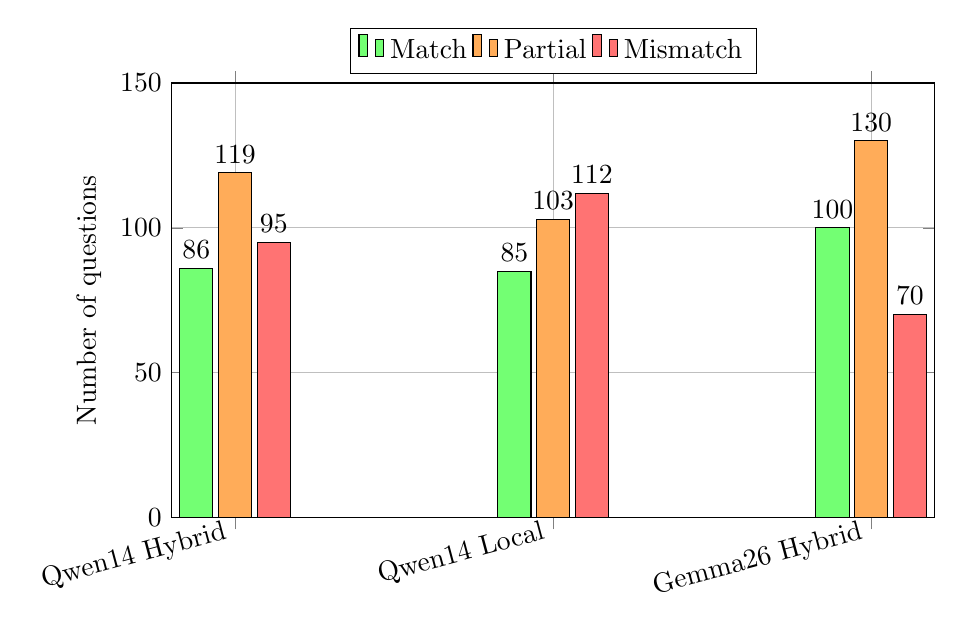
\begin{tikzpicture}
\begin{axis}[
    ybar,
    width=0.93\textwidth,
    height=7.1cm,
    bar width=12pt,
    ylabel={Number of questions},
    symbolic x coords={Qwen14 Hybrid,Qwen14 Local,Gemma26 Hybrid},
    xtick=data,
    x tick label style={rotate=15,anchor=east},
    ymin=0,
    ymax=150,
    legend style={at={(0.5,1.02)},anchor=south,legend columns=3},
    nodes near coords,
    nodes near coords align={vertical},
    grid=major
]
\addplot[fill=green!55] coordinates {(Qwen14 Hybrid,86) (Qwen14 Local,85) (Gemma26 Hybrid,100)};
\addplot[fill=orange!65] coordinates {(Qwen14 Hybrid,119) (Qwen14 Local,103) (Gemma26 Hybrid,130)};
\addplot[fill=red!55] coordinates {(Qwen14 Hybrid,95) (Qwen14 Local,112) (Gemma26 Hybrid,70)};
\legend{Match,Partial,Mismatch}
\end{axis}
\end{tikzpicture}
\caption{Outcome distribution for the three completed configurations.}
\label{fig:outcomes}
\end{figure}

Gemma26 Hybrid achieved the strongest observed result: 14 more matches and 25 fewer mismatches than Qwen14 Hybrid. Qwen14 All-Local achieved almost the same exact-match count as Qwen14 Hybrid, but produced 17 more mismatches. Thus, GPT-5.2 planning and SPARQL generation improved Qwen robustness more than exact-match accuracy.

\subsection{Paired Comparisons}

\begin{table}[H]
\centering
\caption{Paired outcome comparison on the same 300 sample rows. ``Better'' uses the ordering Match $>$ Partial $>$ Mismatch $>$ Crash.}
\label{tab:paired}
\begin{tabular}{lrrr}
\toprule
\textbf{Comparison} & \textbf{First Better} & \textbf{Second Better} & \textbf{Same Grade}\\
\midrule
Qwen14 Hybrid vs.\ Qwen14 All-Local & 55 & 34 & 211\\
Gemma26 Hybrid vs.\ Qwen14 Hybrid & 68 & 49 & 183\\
\bottomrule
\end{tabular}
\end{table}

For Gemma26 versus Qwen14 Hybrid, 29 Qwen mismatches became Gemma matches, 26 became Gemma partials, and 13 Qwen partials became Gemma matches. Conversely, Qwen converted 9 Gemma mismatches to matches, 19 Gemma partials to matches, and 21 Gemma mismatches to partials.

\subsection{Reliability and Self-Healing}

\begin{table}[H]
\centering
\caption{Execution reliability and recovery metrics.}
\label{tab:reliability}
\begin{tabular}{lrrrrr}
\toprule
\textbf{Configuration} & \textbf{Scan Errors} & \textbf{Self-Heal Rows} &
\textbf{Mean Attempts} & \textbf{No-Data/Error} & \textbf{Mean Time (s)}\\
\midrule
Qwen14 Hybrid & 61 & 184 & 1.44 & 77 & 72.92\\
Qwen14 All-Local & 46 & 167 & 1.29 & 100 & 88.73\\
Gemma26 Hybrid & \textbf{21} & \textbf{97} & \textbf{0.67} & \textbf{57} & 74.07\\
\bottomrule
\end{tabular}
\end{table}

\begin{figure}[H]
\centering
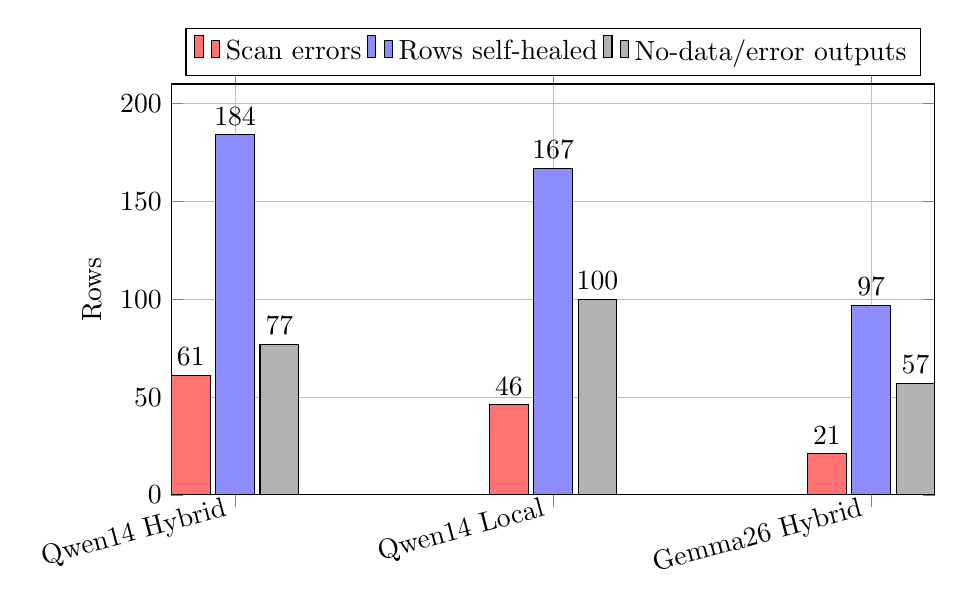
\begin{tikzpicture}
\begin{axis}[
    ybar,
    width=0.93\textwidth,
    height=6.8cm,
    bar width=14pt,
    ylabel={Rows},
    symbolic x coords={Qwen14 Hybrid,Qwen14 Local,Gemma26 Hybrid},
    xtick=data,
    x tick label style={rotate=15,anchor=east},
    ymin=0,
    ymax=210,
    legend style={at={(0.5,1.02)},anchor=south,legend columns=3},
    nodes near coords,
    grid=major
]
\addplot[fill=red!55] coordinates {(Qwen14 Hybrid,61) (Qwen14 Local,46) (Gemma26 Hybrid,21)};
\addplot[fill=blue!45] coordinates {(Qwen14 Hybrid,184) (Qwen14 Local,167) (Gemma26 Hybrid,97)};
\addplot[fill=gray!60] coordinates {(Qwen14 Hybrid,77) (Qwen14 Local,100) (Gemma26 Hybrid,57)};
\legend{Scan errors,Rows self-healed,No-data/error outputs}
\end{axis}
\end{tikzpicture}
\caption{Reliability indicators. Gemma26 Hybrid required substantially fewer repair operations.}
\label{fig:reliability}
\end{figure}

Although the hybrid Qwen run used GPT-5.2 for planning and SPARQL, it still required self-healing on 184 rows. Gemma reduced this to 97 despite using the same GPT-5.2 planning and generation roles. This suggests that semantic operators---particularly Retrieve, Classify, Validate, and Explain---materially affected whether execution was accepted, retried, or translated into a usable answer.

\subsection{Latency}

\begin{table}[H]
\centering
\caption{Per-query latency.}
\label{tab:latency}
\begin{tabular}{lrr}
\toprule
\textbf{Configuration} & \textbf{Mean (s)} & \textbf{Median (s)}\\
\midrule
Qwen14 Hybrid & 72.92 & 63.99\\
Qwen14 All-Local & 88.73 & 81.17\\
Gemma26 Hybrid & 74.07 & \textbf{56.92}\\
\bottomrule
\end{tabular}
\end{table}

The all-local Qwen pipeline was slowest because the local model performed planning, DAG conversion, DAG evaluation, SPARQL generation, and semantic operations. Gemma's mean latency was close to Qwen Hybrid, while its lower median suggests that fewer self-healing rounds offset the larger local model for many questions.

\section{Failure Analysis}

\subsection{Identifier and Alias Failures}

Generated queries sometimes used \texttt{INV01}, \texttt{INV-001}, or \texttt{INV1} when the RDF graph contained \texttt{INV001}. Before alias expansion, only selected forms were resolvable. The RDF-derived map now normalizes all safe zero-padding variants. This optimization should be reevaluated in a controlled rerun because some completed reports predate the final 200-key alias map.

\subsection{Schema and Relationship Hallucination}

Models occasionally selected plausible but nonexistent RDF predicates or reversed relationship directions. Term validation detected unknown \texttt{ex:} terms, but a syntactically valid query could still return zero rows if the relationship semantics were wrong. Better schema slices, explicit relationship metadata, and query execution examples are likely to improve this failure mode.

\subsection{Ties and Incomplete Answers}

Questions such as ``which source handles the most transactions'' can have multiple tied answers. Several generated queries used \texttt{LIMIT 1}, yielding one correct row but omitting equally valid rows. These cases were graded Partial. Future prompts should detect ties or use a two-stage aggregate pattern that returns all maxima/minima.

\subsection{Explanation Loss}

Even when Scan returned correct rows, Explain sometimes omitted IDs, labels, or secondary fields required by the ground truth. This was a major source of Partial outcomes. A schema-aware answer contract or deterministic rendering path could preserve all requested fields without abandoning natural-language explanation.

\subsection{Grading Artifacts}

The deterministic grader occasionally marked a fully correct prose answer Partial because commas or conjunctions were interpreted as extra list items. Conversely, ``no data'' can be considered Match when the ground truth explicitly indicates no rows. These behaviors mean that reported statuses are useful but not equivalent to expert human judgment.

\section{Discussion}

\subsection{Why GPT-5.2 Did Not Produce a Large Exact-Match Gain}

Qwen14 Hybrid achieved only one more Match than Qwen14 All-Local (86 versus 85), although it reduced mismatches by 17. This indicates that GPT-5.2 primarily converted complete failures into partial answers. Model capability alone could not correct incomplete schema retrieval, relationship ambiguity, ties, missing labels, explanation loss, or grading artifacts.

\subsection{Why Gemma26 Hybrid Performed Better}

Gemma26 Hybrid and Qwen14 Hybrid shared GPT-5.2 planning and SPARQL generation, isolating a substantial portion of the difference to local semantic operators. Gemma produced fewer scan errors, fewer no-data/error outputs, and roughly half as many mean self-healing attempts. Possible explanations include stronger schema interpretation, more reliable validation, and better answer synthesis. However, the final graders differed, so this is not a pure model-only comparison.

\subsection{When a Knowledge Graph is Justified}

Many evaluation questions are conventional aggregations that SQL can answer directly. The KG+AOP approach is most justified when the task requires:

\begin{itemize}[leftmargin=*]
    \item semantic integration across heterogeneous sources;
    \item explicit entity and relationship traversal;
    \item ontology-based validation and explainability;
    \item alias and entity-resolution support;
    \item schema evolution; or
    \item multi-hop reasoning not easily captured by a single known relational query.
\end{itemize}

Accordingly, a direct text-to-SQL baseline is necessary before claiming practical superiority.

\section{Threats to Validity}

\begin{enumerate}[leftmargin=*]
    \item \textbf{Non-uniform grading.} Qwen14 Hybrid used Qwen32 for unresolved final grading, while Gemma26 Hybrid used Gemma26 itself.
    \item \textbf{Alias-map timing.} The expanded RDF alias map was introduced during the experiment timeline; not every report was generated under the same map.
    \item \textbf{Misleading metadata.} The Gemma CSV inherited a Qwen-named pipeline-version string from \texttt{.env}. Runtime inspection confirmed Gemma execution, but the metadata should be corrected.
    \item \textbf{Previously failed sample.} The 300 questions are not an unbiased test set; they were selected because a prior pipeline marked them Mismatch.
    \item \textbf{Duplicate questions.} The set includes 68 duplicate rows, which can overweight recurring query templates.
    \item \textbf{Automated grading noise.} Known false Partial classifications and model-based grader variability remain.
    \item \textbf{Hybrid confounding.} Planner, generator, semantic operator, and grader changes are not independently ablated in all configurations.
\end{enumerate}

\section{Future Work}

\subsection{Controlled Model Ablations}

Run a factorial experiment where exactly one role changes at a time:

\begin{enumerate}[leftmargin=*]
    \item fixed DAG and schema slice, vary only SPARQL model;
    \item fixed SPARQL, vary only Explain;
    \item fixed planner and generator, vary Retrieve/Classify/Validate;
    \item fixed outputs, use one independent grader for all configurations.
\end{enumerate}

\subsection{Baselines}

Future evaluation should include:

\begin{itemize}[leftmargin=*]
    \item direct text-to-SQL over the original relational tables;
    \item direct one-shot text-to-SPARQL without AOP;
    \item fixed deterministic operator chain;
    \item AOP without self-healing;
    \item AOP without alias preprocessing; and
    \item oracle schema retrieval.
\end{itemize}

\subsection{Human Evaluation}

At least two annotators should independently review a stratified sample of Match, Partial, and Mismatch rows. Inter-annotator agreement and adjudicated labels would quantify grader noise and establish a more defensible accuracy estimate.

\subsection{Query-Structure Metrics}

Beyond final answers, evaluate:

\begin{itemize}[leftmargin=*]
    \item SPARQL parse success;
    \item vocabulary grounding precision;
    \item correct relationship direction;
    \item execution success;
    \item row-level precision and recall;
    \item tie completeness;
    \item DAG validity on first attempt;
    \item number of LLM calls and tokens;
    \item GPU time, API cost, and energy; and
    \item self-healing success rate by error category.
\end{itemize}

\subsection{Hybrid SQL--SPARQL Routing}

A future planner could choose between SQL and SPARQL:

\begin{figure}[H]
\centering
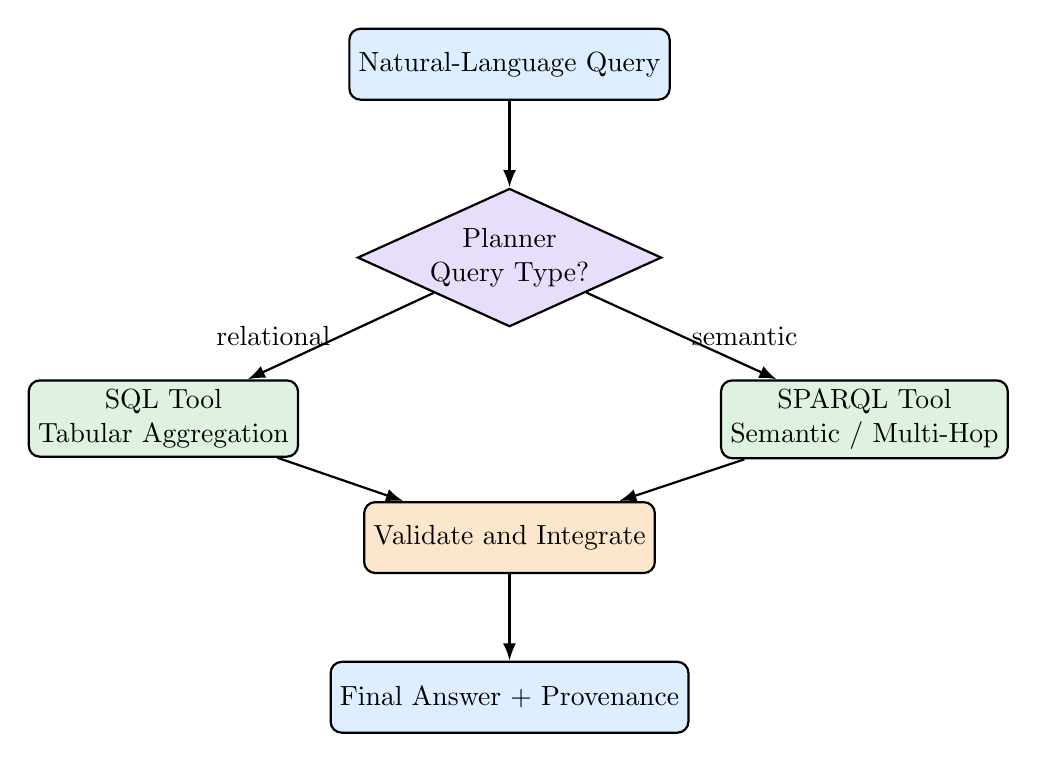
\begin{tikzpicture}[
    node distance=11mm and 17mm,
    box/.style={rectangle, rounded corners, draw, thick, align=center, minimum height=9mm, minimum width=27mm},
    decision/.style={diamond, draw, thick, align=center, aspect=2.2, inner sep=1pt},
    arrow/.style={-{Latex[length=2.2mm]}, thick}
]
\node[box, fill=inputblue] (q) {Natural-Language Query};
\node[decision, fill=planpurple, below=of q] (route) {Planner\\Query Type?};
\node[box, fill=execgreen, below left=of route] (sql) {SQL Tool\\Tabular Aggregation};
\node[box, fill=execgreen, below right=of route] (sparql) {SPARQL Tool\\Semantic / Multi-Hop};
\node[box, fill=checkorange, below=22mm of route] (integrate) {Validate and Integrate};
\node[box, fill=inputblue, below=of integrate] (answer) {Final Answer + Provenance};
\draw[arrow] (q) -- (route);
\draw[arrow] (route) -- node[left]{relational} (sql);
\draw[arrow] (route) -- node[right]{semantic} (sparql);
\draw[arrow] (sql) -- (integrate);
\draw[arrow] (sparql) -- (integrate);
\draw[arrow] (integrate) -- (answer);
\end{tikzpicture}
\caption{Proposed hybrid SQL--SPARQL architecture.}
\label{fig:future}
\end{figure}

This design preserves KG benefits for relationship-centric questions while using SQL for straightforward aggregation.

\section{Conclusion}

This study implemented and evaluated a modular agent-oriented pipeline for financial KG question answering. The system combines LLM-planned DAGs, RDF-derived schema retrieval, SPARQL generation, deterministic graph execution, validation, alias normalization, and self-healing. Among the completed configurations, Gemma26 Hybrid achieved the strongest outcome, with 100 matches and 70 mismatches on 300 previously failed questions. The results also show that stronger models alone do not eliminate failures: schema grounding, identifier normalization, tie handling, answer preservation, and evaluation design remain major bottlenecks.

The principal research contribution is therefore not a claim that KG+AOP universally outperforms SQL. Rather, it is a detailed account of how modular language-model agents interact with a semantic graph execution layer, which optimizations improve robustness, and which failure modes must be controlled before such systems can be evaluated or deployed reliably.

\begin{thebibliography}{99}

\bibitem{shoham1993aop}
Y. Shoham,
``Agent-Oriented Programming,''
\emph{Artificial Intelligence}, vol. 60, no. 1, pp. 51--92, 1993.
doi: 10.1016/0004-3702(93)90034-9.

\bibitem{rdf11}
R. Cyganiak, D. Wood, and M. Lanthaler,
``RDF 1.1 Concepts and Abstract Syntax,''
W3C Recommendation, 2014.
\url{https://www.w3.org/TR/rdf11-concepts/}

\bibitem{sparql11}
S. Harris and A. Seaborne,
``SPARQL 1.1 Query Language,''
W3C Recommendation, 2013.
\url{https://www.w3.org/TR/sparql11-query/}

\bibitem{hogan2021kg}
A. Hogan, E. Blomqvist, M. Cochez, C. d'Amato, G. de Melo, C. Gutierrez,
S. Kirrane, J. E. L. Gayo, R. Navigli, S. Neumaier, A.-C. N. Ngomo,
A. Polleres, S. M. Rashid, A. Rula, L. Schmelzeisen, J. Sequeda,
S. Staab, and A. Zimmermann,
``Knowledge Graphs,''
\emph{ACM Computing Surveys}, vol. 54, no. 4, Article 71, 2021.
doi: 10.1145/3447772.

\bibitem{yao2023react}
S. Yao, J. Zhao, D. Yu, N. Du, I. Shafran, K. Narasimhan, and Y. Cao,
``ReAct: Synergizing Reasoning and Acting in Language Models,''
in \emph{International Conference on Learning Representations}, 2023.
\url{https://arxiv.org/abs/2210.03629}

\bibitem{madaan2023selfrefine}
A. Madaan, N. Tandon, P. Gupta, S. Hallinan, L. Gao, S. Wiegreffe,
U. Alon, N. Dziri, S. Prabhumoye, Y. Yang, S. Welleck, B. P. Majumder,
S. Gupta, A. Yazdanbakhsh, and P. Clark,
``Self-Refine: Iterative Refinement with Self-Feedback,''
in \emph{Advances in Neural Information Processing Systems}, 2023.
\url{https://arxiv.org/abs/2303.17651}

\bibitem{yu2018spider}
T. Yu, R. Zhang, K. Yang, M. Yasunaga, D. Wang, Z. Li, J. Ma,
I. Li, Q. Yao, S. Roman, Z. Zhang, and D. Radev,
``Spider: A Large-Scale Human-Labeled Dataset for Complex and Cross-Domain
Semantic Parsing and Text-to-SQL Task,''
in \emph{Proceedings of EMNLP}, 2018.
\url{https://aclanthology.org/D18-1425/}

\end{thebibliography}

\appendix

\section{Reproducibility Checklist}

\begin{itemize}[leftmargin=*]
    \item Input sample: \texttt{random\_300\_mismatch.csv}
    \item RDF schema: \texttt{schema\_linkage\_graph\_v2.rdf}
    \item RDF instances: \texttt{business\_data\_kg\_schema\_aligned.ttl}
    \item Alias map: \texttt{rdf\_id\_alias\_map.json}
    \item Main reports:
    \begin{itemize}
        \item \texttt{Pipeline\_Retest\_Report\_qwen14b.csv}
        \item \texttt{Pipeline\_Retest\_Report\_qwen14b\_all\_local.csv}
        \item \texttt{Pipeline\_Retest\_Report\_gemma4\_26b.csv}
    \end{itemize}
    \item Local runtime: Ollama OpenAI-compatible endpoint on port 11440
    \item Graph execution: RDFLib
    \item DAG representation and validation: NetworkX
\end{itemize}

\section{Recommended Next Experiment Matrix}

\begin{table}[H]
\centering
\small
\caption{Suggested controlled ablation matrix.}
\begin{tabular}{lllll}
\toprule
\textbf{Run} & \textbf{Planner} & \textbf{SPARQL} & \textbf{Semantic Ops} & \textbf{Purpose}\\
\midrule
A & GPT-5.2 & GPT-5.2 & Qwen14 & Existing hybrid baseline\\
B & GPT-5.2 & Qwen14 & Qwen14 & Isolate SPARQL model\\
C & Qwen14 & GPT-5.2 & Qwen14 & Isolate planner model\\
D & GPT-5.2 & GPT-5.2 & Gemma26 & Existing Gemma hybrid\\
E & Fixed DAG & GPT-5.2 & Qwen14 & Remove planning variance\\
F & Fixed DAG & Qwen14 & Qwen14 & SPARQL-only comparison\\
G & Text-to-SQL & SQL execution & Fixed renderer & Relational baseline\\
\bottomrule
\end{tabular}
\end{table}

\end{document}
